%\newpage
\section{Multinomial Models}

    \subsection{Naïve Multinomial Model}
        Naïve estimations of multinomial logit
        \begin{align}
            \mathbb{P}(\texttt{party} = j\vert z) = F_j(z'\beta), \quad j \in \{\texttt{CDU}/\texttt{CSU}, \texttt{SPD}, \texttt{GREENS} \}
            \label{multi_model_1}
        \end{align}
        is presented in Table \ref{tab_21_naivelogit}. Now the estimated effects are for the probability to vote either SPD or The Greens compared to the probability of voting for CDU/CSU. The estimates are the Relative Risk Ratios (RRR) which is the natural generalization of the odds ratio. Hence, e.g. females is more likely to vote for the The Greens than men relative (by 1.39 times) compared to voting for CDU/CSU everything else held constant.
        \begin{samepage}
                \begin{table}[]
                    \footnotesize
                    \centering
                    \subfile{tabs/21_naivelogit}
                    \caption{Naïve Multinomial Logit}
                    \label{tab_21_naivelogit}
                \end{table}
            \end{samepage}
    
    \subsection{Means Marginal Effects}
        Marginal effects at the mean for females is presented in Figure \ref{fig_22_female}. It is seen that females are less likely to vote for CDU/CSU (Category 1) or SPD (Category 2) than males. They are more likely to vote for The Greens.
            \begin{figure}[!htb]
                \centering
                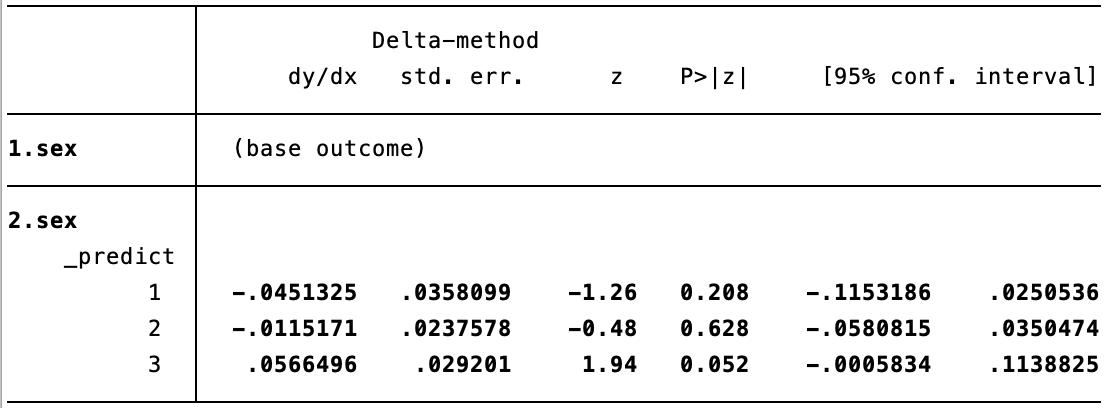
\includegraphics[width=10cm]{figs/22_female.png}
                \caption{Marginal Effects of Naïve Multinomial Logit for Females at the Mean}
                \label{fig_22_female}
            \end{figure}
            \begin{figure}[!htb]
                \centering
                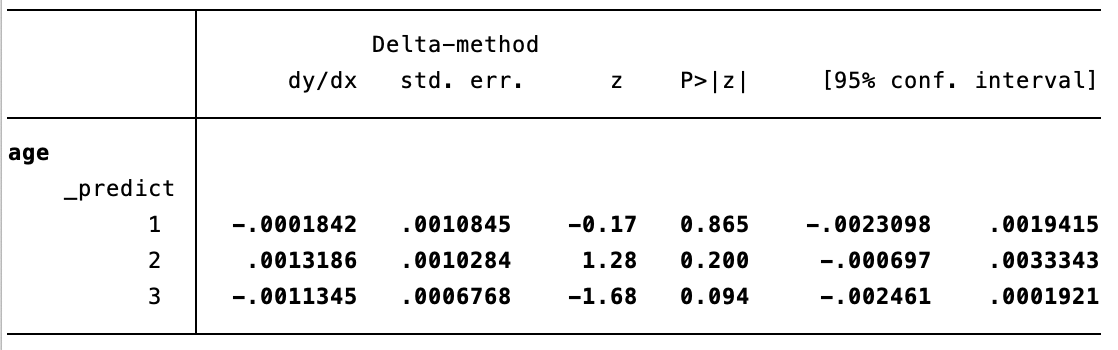
\includegraphics[width=10cm]{figs/22_age.png}
                \caption{Marginal Effects of Naïve Multinomial Logit for Age at the Mean}
                \label{fig_22_age}
            \end{figure}
        \newline\indent
        Given that the population is ageing I would expect higher age to be associated to vote for one of the centrist parties (CDU/CSU or SPD). Running marginal effects for age is presented in Figure \ref{fig_22_age}. This confirms that an increase in age is associated with higher probability to vote for SPD (Category 2), but is (surprisingly) associated with lower probability to vote for CDU/CSU. Unsurprisingly, older people are less likely to vote for the progressive The Greens. 
    
    %\newpage
    \begin{samepage}
        \subsection{Manual Estimation}
        As in Section \ref{subsec_bin_man_est}, the code snippet below is developed in cooperation with Manohar Gannavarapu and John Searight as allowed by Prof. Wang.
            \begin{verbatim}
program define my_multi_logit
    args lnf Xb2 Xb3
    quietly replace `lnf' = - ln(1+exp(`Xb2')+exp(`Xb3')) if $ML_y1==1
    quietly replace `lnf' = `Xb2' - ln(1+exp(`Xb2')+exp(`Xb3')) if $ML_y1==2
    quietly replace `lnf' = `Xb3' - ln(1+exp(`Xb2')+exp(`Xb3')) if $ML_y1==4
end

ml model lf my_multi_logit (xb2:pv01= $regressors) (xb3:= $regressors)
ml maximize
            \end{verbatim}
    which outputs numerically equivalent estimations as Table \ref{tab_21_naivelogit} with coefficients instead of risk-relative ratios (see Figure \ref{fig_a2_multi1_coefs}).
    \end{samepage}
    
    
    \subsection{Conditional Logit}
    The output from the conditional logit model is presented in Table \ref{tab_24_condlogit}. Please refer to the attached \texttt{.do}-file for the data wrangling part necessary for Stata's \texttt{asclogit} command. The alternative-varying variable is the party to vote for (\texttt{options}) and the case-specific variables are \texttt{sex}, \texttt{age}, \texttt{educ} and \texttt{work}. The outcome is the party chosen (\texttt{y}) while the alternative-specific is the distance between the voter's own political views to the party’s position on the left-to-right spectrum (\texttt{distance}).
        \begin{samepage}
                \begin{table}[]
                    \footnotesize
                    \centering
                    \subfile{tabs/24_condlogit}
                    \caption{Conditional Logit}
                    \label{tab_24_condlogit}
                \end{table}
            \end{samepage}
    \newline\indent
    I interpret the negative sign for \texttt{distance} such that if the distance between individuals' own views and the position of the party on the left-right scale increases, on average individuals will tend to vote less for that party and more for the other options.
    
    
    \subsection{Extended Multinomial Logit}
        Table \ref{tab_25_mlogit} presents estimation of regression model \eqref{multi_model_1} but with the addition of respondents’ own position on the left-right spectrum, i.e. \texttt{pa01}. \texttt{pa01} is coded as an ordered categorical variable with higher values signifying more right-leaning subjective political views. 
            \newline\indent
        More right-leaning views are associated with higher likelihood of voting for FDP and (even more) for AFD compared to CDU/CSU. This is unsurprising since AFD is the most right-leaning party and FDP is a free-market party (I believe without being an expert). 
            \newline\indent
        More left-leaning views makes it more likely to vote SPD and The Greens which are centrist-left and progressive, respectively. It makes it the most unlikely to vote for The Left which is the most left-leaning party so this is also unsurprising.
            \begin{landscape}
                        \begin{table}[]
                            \footnotesize
                            \centering
                            \subfile{tabs/25_mlogit}
                            \caption{Extended Multinomial Logit}
                            \label{tab_25_mlogit}
                        \end{table}
                \end{landscape}
    
    
    \subsection{Nested Logit}
    The tree structure of the nested logit model is shown in Figure \ref{fig_27_tree}. The output from the regression is shown in Table \ref{tab_26_nlogit}.
        \begin{figure}[!htb]
                \centering
                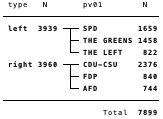
\includegraphics[width=5cm]{figs/27_tree}
                \caption{Nested Logit Tree Structure}
                \label{fig_27_tree}
            \end{figure} 
            \begin{landscape}
                \begin{table}[]
                    \scriptsize
                    \centering
                    \subfile{tabs/26_nlogit}
                    \caption{Nested Logit}
                    \label{tab_26_nlogit}
                \end{table}
            \end{landscape}
            
            
            
            
            
            
    
    \subsection{Experimentation}
    Due to the long run time of the \texttt{nlogit} command I have only been able to estimate  acouple of multinomial logit models. 
    
    \paragraph{Table \ref{tab_27_model1}} Environmental protection sentiment is added as a regressor. It indicates the level of disagreement to whether environmental protection policies should be stricter. The results show that if a respondent disagrees they are more likely (compared to voting for CDU/CSU) to vote for
    \begin{itemize}
        \item FDP: I think FDP is a free-market party so I suppose it would make sense that environmentalists would favor other parties.
        \item AFD: I think this makes sense as the party is more conservative.
    \end{itemize}
    and less likely (relative to CDU/CSU) to vote for
    \begin{itemize}
        \item SPD: This makes sense, since it is the centre-left party.
        \item The Left: Unsurprising, since it is the most progressive party.
        \item Greens: Unsurprising, because even the party's name suggests that environmental policies are very important for this party.
    \end{itemize}
    
    
    \paragraph{Table \ref{tab_27_model2}}
    Immigrant sentiment is added as a regressor. It indicates the level of disagreement to whether immigrants are good for the German economy. The results show that if a respondent disagrees they are more likely (compared to voting for CDU/CSU) to vote for
    \begin{itemize}
        \item FDP: I do not have enough insider knowledge to evaluate if this makes sense.
        \item The Left: This is surprising given the progressive ideology of this party but the results are also not significant.
        \item AFD: This makes sense since the party is very anti-immigrant. The effect is highly significant as well.
    \end{itemize}
    and less likely (relative to CDU/CSU) to vote for
    \begin{itemize}
        \item SPD: Unsurpring, since it is the centre-left party.
        \item Greens: Unsurprising, since it is a progressive party.
    \end{itemize}
    
    \paragraph{Table \ref{tab_27_model3}}
    Newspaper Exposure is added as a regressor. It is a ordered variable indicating how many days a week a recipient reads the newspaper, i.e. $\in\{0,1,...,7\}$. Higher newspaper exposure is associated with less probability to vote for all other parties compared to CDU/CSU. However, the highest effects in magnitude are for The Left and AFD. This seems reasonable as they are the most extreme parties on the left-right spectrum. Thus, it would make sense that their voters read less newspapers (and perhaps get their news from e.g. Facebook instead). These effects are also the only ones that are statistically significant.
        
        \newpage
            \begin{samepage}
                \begin{landscape}
                        \begin{table}[]
                            \footnotesize
                            \centering
                            \subfile{tabs/27_model1}
                            \caption{Same as Table \ref{tab_21_naivelogit} + Environmental Protection Sentiment}
                            \label{tab_27_model1}
                        \end{table}
                \end{landscape}
            \end{samepage}
        \newpage
            \begin{samepage}
                \begin{landscape}
                        \begin{table}[]
                            \footnotesize
                            \centering
                            \subfile{tabs/27_model2}
                            \caption{Same as Table \ref{tab_21_naivelogit} + Immigrant Sentiment}
                            \label{tab_27_model2}
                        \end{table}
                \end{landscape}
            \end{samepage}
        \newpage
            \begin{samepage}
                \begin{landscape}
                        \begin{table}[]
                            \footnotesize
                            \centering
                            \subfile{tabs/27_model3}
                            \caption{Same as Table \ref{tab_21_naivelogit} + Newspaper Exposure}
                            \label{tab_27_model3}
                        \end{table}
                \end{landscape}
            \end{samepage}
